\chapter{Results}

\section{Experiment 1}
Experiment~1 tests the role of prosody in intelligibility, by comparing mean sentence scores for unmodified talkers against resynthesized stimuli with prosodic replacement.  The mean sentence score for each talker across listeners is shown in Figure~\ref{fig:ExpOneBarplot}.  Darker bars indicate unmodified recordings, while light bars represent resynthesized stimuli.  Contrary to expectations, not all resynthesized stimuli have lower mean scores compared to their unmodified counterparts, suggesting that distortion due to the resynthesis process was relatively minimal.\footnotemark{}  With regard to Research Question~1 — how does prosody relate to intelligibility — a complicated picture emerges.  Talker~\ac{b} suffers dramatically when his prosody is replaced, whereas Talker~\ac{c} is unchanged or slightly improved, and Talker~\ac{a} is unchanged or slightly worsened.

\footnotetext{This is likely due to several factors.  One is probably the painstaking hand-correction of the pulse marking to ensure consistent phase throughout voiced spans of speech.  Another is the choice to maintain each talker’s natural mean pitch on each sentence, and map only the {\emph shape} of the pitch contour of the prosodic donor during resynthesis.}

One possible explanation for these results is to postulate that Talker~\ac{a}, despite being highly intelligible, does not have especially good prosody, evidenced in particular by the fact that scores for Talker~\ac{ca} are lower than the scores for Talker~\ac{cb}.  On the same grounds, and on the additional observation that scores for Talker~\ac{ab} are greater than for Talker~\ac{ac}, we might conclude that Talker~\ac{b} has more intelligible prosody than the other two talkers, and his middling base intelligibility scores are due to segmental factors.

\begin{figure}[htbp]
	\begin{centering}
	\includegraphics{figures/results/ExpOneBarplot.eps}
	\caption[Barplot of mean sentence scores for Experiment~1]{Barplot of mean sentence scores for Experiment~1.  Error bars are ±1 standard error; lighter colors indicate resynthesized talkers, with the second letter indicating the prosodic donor (see Section~\ref{sec:ExpDesign} for full explanation of talker codes).\label{fig:ExpOneBarplot}}
	\end{centering}
\end{figure}

With regard to the question of whether low-intelligibility talkers can be made more intelligible through prosody alone, it would appear that the answer is “yes”: Talker~\ac{cb} appears to have higher scores than Talker~\ac{c}, despite the likelihood that Talker~\ac{cb}’s recordings suffer some amount of distortion from the resynthesis process.  In other words, any detriment due to resynthesis is more than overcome by the benefit of having Talker~\ac{b}’s prosody.  

To further probe these results, the scores were submitted to a mixed-effects linear regression model, shown in Equation~\ref{eq:ExpOneMM}:

\begin{equation}\label{eq:ExpOneMM}
	\text{{\inlinecode lmer(sentScore\textasciitilde resynth+segDonor+proDonor+(1|listener)+(1|sentence), data=allData)}}
\end{equation}

In this model, {\inlinecode sentScore} is the number of keywords correct (0–5), {\inlinecode resynth} is a boolean variable that is true for Talkers~\ac{ab ac ba bc ca} and~\ac{cb}, and {\inlinecode segDonor} and {\inlinecode proDonor} are three-level factors indicating the talker in the target signal and the talker from whom the prosodic information was drawn, respectively.  For the unmodified original recordings, {\inlinecode segDonor} and {\inlinecode proDonor} are defined as the talker himself, even though those recordings were not resynthesized.  

A summary of the model shown in Equation~\ref{eq:ExpOneMM} is given in Table~\ref{tab:ExpOneFixedEff}.  There was no evidence of correlation of fixed effects (correlation coefficients ranged from 0 to 0.505; not shown in Table~\ref{tab:ExpOneFixedEff}).  The baseline condition is Talker~\ac{a}, with a value at the intercept of about 4.4 words correct.  The coefficients reveal similar patterns as Figure~\ref{fig:ExpOneBarplot}.  Firstly, the model supports the interpretation that Talker~\ac{b} has the most intelligible prosody: having the prosody of Talker~\ac{b} represents a net gain of 0.3 words correct over the prosody of Talker~\ac{a}, whereas having the prosody of Talker~\ac{c} represents a net loss of 0.6 words correct.  The model also supports the idea that Talker~\ac{a}’s intelligibility stems in large part from segmental factors, given that the other levels of {\inlinecode segDonor} both have strongly negative coefficients.

% TODO: fix rowfont bolding (currently not bolding) in this table and in Exp 2 table
\begin{table}
	\caption[Experiment~1 statistical model: Fixed effects]{Summary of fixed effect predictors in the statistical model of Experiment~1.\label{tab:ExpOneFixedEff}}
	\centering
	\begin{tabu} spread 1em {Xrcrc}
		\toprule
		\rowfont{\textbf}\multicolumn{5}{l}{Summary of fixed effects (N=1440; log-likelihood=-2554)}\\
		\rowfont[c]{\textbf}\multicolumn{1}{l}{Predictor} & Coefficient & \textit{SE} & \textit{t} & \textit{p}\\
		\midrule
		Intercept         &  4.382 & (0.132) &  33.19 & <10⁻¹⁶\\
		resynth = TRUE    & −0.666 & (0.077) &  −8.64 & <10⁻¹⁶\\
		segDonor = \ac{b} & −1.679 & (0.089) & −18.82 & <10⁻¹⁶\\
		segDonor = \ac{c} & −1.274 & (0.090) & −14.18 & <10⁻¹⁶\\
		proDonor = \ac{b} &  0.315 & (0.089) &   3.54 & <10⁻³\\
		proDonor = \ac{c} & −0.635 & (0.088) &  −7.19 & <10⁻¹¹\\
		\bottomrule
	\end{tabu}
\end{table}

A summary of the random effects in the model of Experiment~1 are shown in Table~\ref{tab:ExpOneRandomEff}.  The results are unremarkable: as expected, the variability of listeners is relatively low (s²=0.043, or a standard deviation of 0.2 keywords correct across listeners), suggesting that to a first approximation listeners are all equally good at the task.  In contrast, the variability of sentence difficulty is somewhat higher (s²=0.513, or a standard deviation of 0.7 keywords correct across sentences).

%Random effects:
% Groups   Name        Variance Std.Dev. MCMCmean   HPD95lower HPD95upper
% sent     (Intercept) 0.51345  0.71655  0.6040129  0.5055609  0.7081530
% listener (Intercept) 0.04289  0.20710  0.2212181  0.1082121  0.3494921
% Residual             1.78542  1.33620  1.3516454  1.3010096  1.4038710
\begin{table}
	\caption[Experiment~1 statistical model: Random effects]{Summary of random effects in the statistical model of Experiment~1.\label{tab:ExpOneRandomEff}}
	\centering
	\begin{tabu} spread 1em {Xcccc}
		\toprule
		\multicolumn{3}{l}{\bfseries Summary of random effects} & \multicolumn{2}{c}{95\% \ac{hpd}}\\
		Group & \textit{s}² & \ac{mcmc} mean & lower bound & upper bound\\
		\midrule
		Sentence (intercept) & (0.513) & 0.604 & 0.506 & 0.708\\
		Listener (intercept) & (0.043) & 0.221 & 0.108 & 0.349\\
		Residual             & (1.785) & 1.352 & 1.301 & 1.404\\
		\bottomrule
	\end{tabu}
\end{table}


\section{Experiment 2}
Experiment~2 tests the role of prosody in the familiar talker advantage, by comparing mean sentence scores for various talkers across two groups of listeners: those trained on one of the test talkers (Talker~\ac{c}), and those trained on a control talker (Talker~\ac{d}).  The first question to be addressed is whether the training phase was in fact effective for both groups of listeners.  Mean sentence scores of the training phase (grouped by quartile) are shown in Figure~\ref{fig:Quartile}. 

\begin{figure}[htbp]
	\begin{centering}
	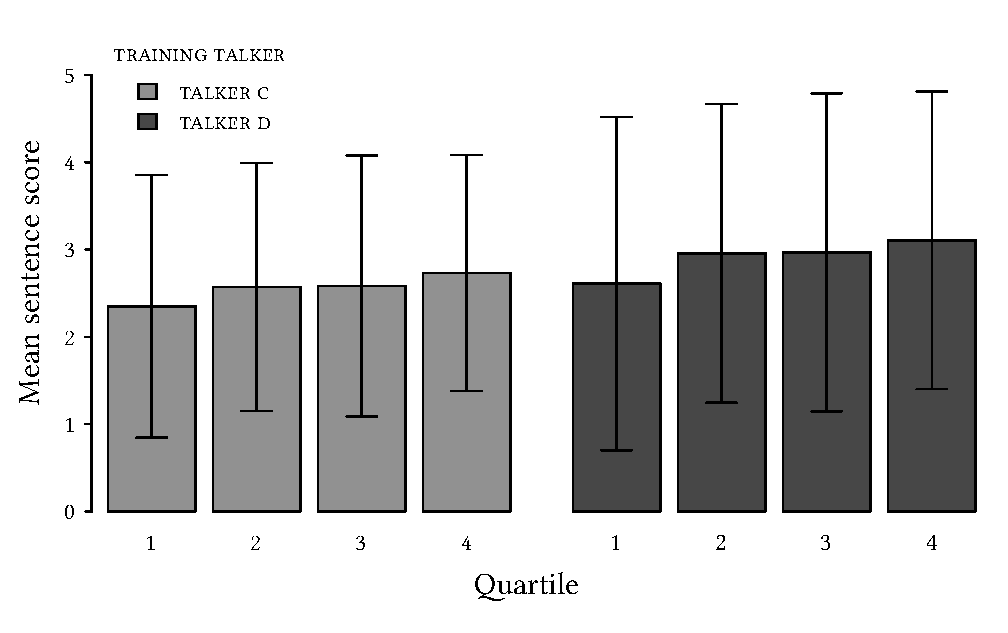
\includegraphics{figures/results/QuartileBarplot.eps}
	\caption[Quartile analysis of training phase in Experiment~2]{Quartile analysis of training phase in Experiment~2.  Improvement is seen during training for both the control group (trained on Talker~\ac{d}) and the test group (trained on Talker~\ac{c}).  The adaptation in the test group appears not to have been maintained during testing.\label{fig:Quartile}}
	\end{centering}
\end{figure}

T-tests performed on the first and fourth quartile of each group show a statistically significant improvement in both groups of listeners (control group: \textit{t}=−2.898 on 437.2 degrees of freedom, \textit{p}<0.01; test group: \textit{t}=−2.816 on 438.1 degrees of freedom, \textit{p}<0.01).  However, the improvement is small (less that 0.5 keywords for both groups), and more importantly it appears the adaptation that occurred during training was not fully retained during the testing phase, as evidenced by the slight decline in performance on Talker~\ac{c} during the testing phase when compared to the last quartile of the training phase (see Figure~\ref{fig:Quartile}).\footnotemark{}

footnotetext{This is true at least for the listeners trained on Talker~\ac{c}.  Listeners trained on Talker~\ac{d} did not hear their training talker during the testing phase, so it is unknown whether any adaptation was retained during testing.  Presumably, however, any such adaptation would have had little effect on performance when listening to Talkers~\ac{a}, \ac{b}, or \ac{c}.}

One explanation for the failure to retain a perceptual advantage between the training to the testing phases is stimulus uncertainty: in the training phase, listeners heard the same talker for 90 sentences in a row, whereas the testing phase comprised a random ordering of sentences from the three unmodified talkers and the six resynthesized talkers.  It is possible that the uncertainty due to varying the talkers negated any advantage acquired from the training.  Another possible explanation is that the training was too brief, and the apparent learning seen in the quartile analysis is merely a task familiarization effect that was not tied to any particular talker.

In light of the preceding discussion it is perhaps unsurprising that training on a particular talker did not confer a reliable perceptual advantage on test stimuli resynthesized to have the training talker’s prosody.  Full results of the statistical model for Experiment~2 are shown in Table~\ref{tab:ExpTwoFixedEff}.  Predictor codes are the same as in the model for Experiment~1, with the addition of {\inlinecode segTrain} (a boolean variable indicating match between the training talker and the segmental donor of the test stimulus) and {\inlinecode proTrain} (indicating match between the training talker and the prosodic donor of the test stimulus).

Aside from the two non-significant predictors {\inlinecode segTrain} and {\inlinecode proTrain}, the model is nearly identical to the model for Experiment~1; the magnitude, direction, and significance of the other predictors are all unchanged from Experiment~1.

\begin{table}
	\caption[Experiment~2 statistical model: Fixed effects]{Summary of fixed effect predictors in the statistical model of Experiment~2.\label{tab:ExpTwoFixedEff}}
	\centering
	\begin{tabu} spread 1em {Xrcrc}
		\toprule
		\rowfont{\textbf}\multicolumn{5}{l}{Summary of fixed effects (N=1800; log-likelihood=-3103)}\\
		\rowfont[c]{\textbf}\multicolumn{1}{l}{Predictor} & Coefficient & \textit{SE} & \textit{t} & \textit{p}\\
		\midrule
		Intercept	      &  4.334 & (0.129) &  33.56 & <10⁻¹⁶\\
		resynth = TRUE    & −0.604 & (0.066) &  −9.17 & <10⁻¹⁶\\
		segDonor = \ac{b} & −1.467 & (0.075) & −19.46 & <10⁻¹⁶\\
		segDonor = \ac{c} & −1.160 & (0.098) & −11.83 & <10⁻¹⁶\\
		proDonor = \ac{b} &  0.269 & (0.075) &   3.59 & <10⁻³\\
		proDonor = \ac{c} & −0.586 & (0.098) &  −5.98 & <10⁻⁸\\
		segTrain = TRUE   &  0.009 & (0.125) &   0.08 & 0.94\\
		proTrain = TRUE   & −0.115 & (0.125) &  −0.92 & 0.36\\
		\bottomrule
	\end{tabu}
\end{table}

A summary of the random effects in the model of Experiment~2 are shown in Table~\ref{tab:ExpTwoRandomEff}.  The results are again unremarkable: like the model for Experiment~1, the variability of listeners is relatively low (s²=0.083, or a standard deviation of 0.3 keywords correct across listeners), and the variability of sentence difficulty is again somewhat higher (s²=0.537, or a standard deviation of 0.7 keywords correct across sentences).

% Random effects:
% Groups   Name        Variance Std.Dev. MCMCmean   HPD95lower HPD95upper
% sent     (Intercept) 0.537497 0.73314  0.6170353  0.5238609  0.7132486
% listener (Intercept) 0.083091 0.28825  0.2972227  0.1879063  0.4192268
% Residual             1.616020 1.27123  1.2835182  1.2405740  1.3280362

\begin{table}
	\caption[Experiment~2 statistical model: Random effects]{Summary of random effects in the statistical model of Experiment~2.\label{tab:ExpTwoRandomEff}}
	\centering
	\begin{tabu} spread 1em {Xcccc}
		\toprule
		\multicolumn{3}{l}{\bfseries Summary of random effects} & \multicolumn{2}{c}{95\% \ac{hpd}}\\
		Group & \textit{s}² & \ac{mcmc} mean & lower bound & upper bound\\
		\midrule
		Sentence (intercept) & (0.537) & 0.617 & 0.524 & 0.713\\
		Listener (intercept) & (0.083) & 0.297 & 0.188 & 0.419\\
		Residual             & (1.616) & 1.284 & 1.241 & 1.328\\
		\bottomrule
	\end{tabu}
\end{table}

% TODO: check mismatch between binary and continuous models for experiment 2

% TODO: some closing remarks?

% TODO: post hoc: count release bursts?
% TODO: post hoc: pitch range, pitch dynamicity, intensity velocity, vowel space area?
% TODO: training with talker B


